\documentclass[border=10pt]{standalone}

\usepackage{tikz}
\usepackage{tikzsymbols}
\usetikzlibrary{calc,patterns,shapes.geometric}

\def\centerarc[#1](#2)(#3:#4:#5){\draw[#1] ($(#2)+({#5*cos(#3)},{#5*sin(#3)})$) arc (#3:#4:#5);}

\begin{document}
	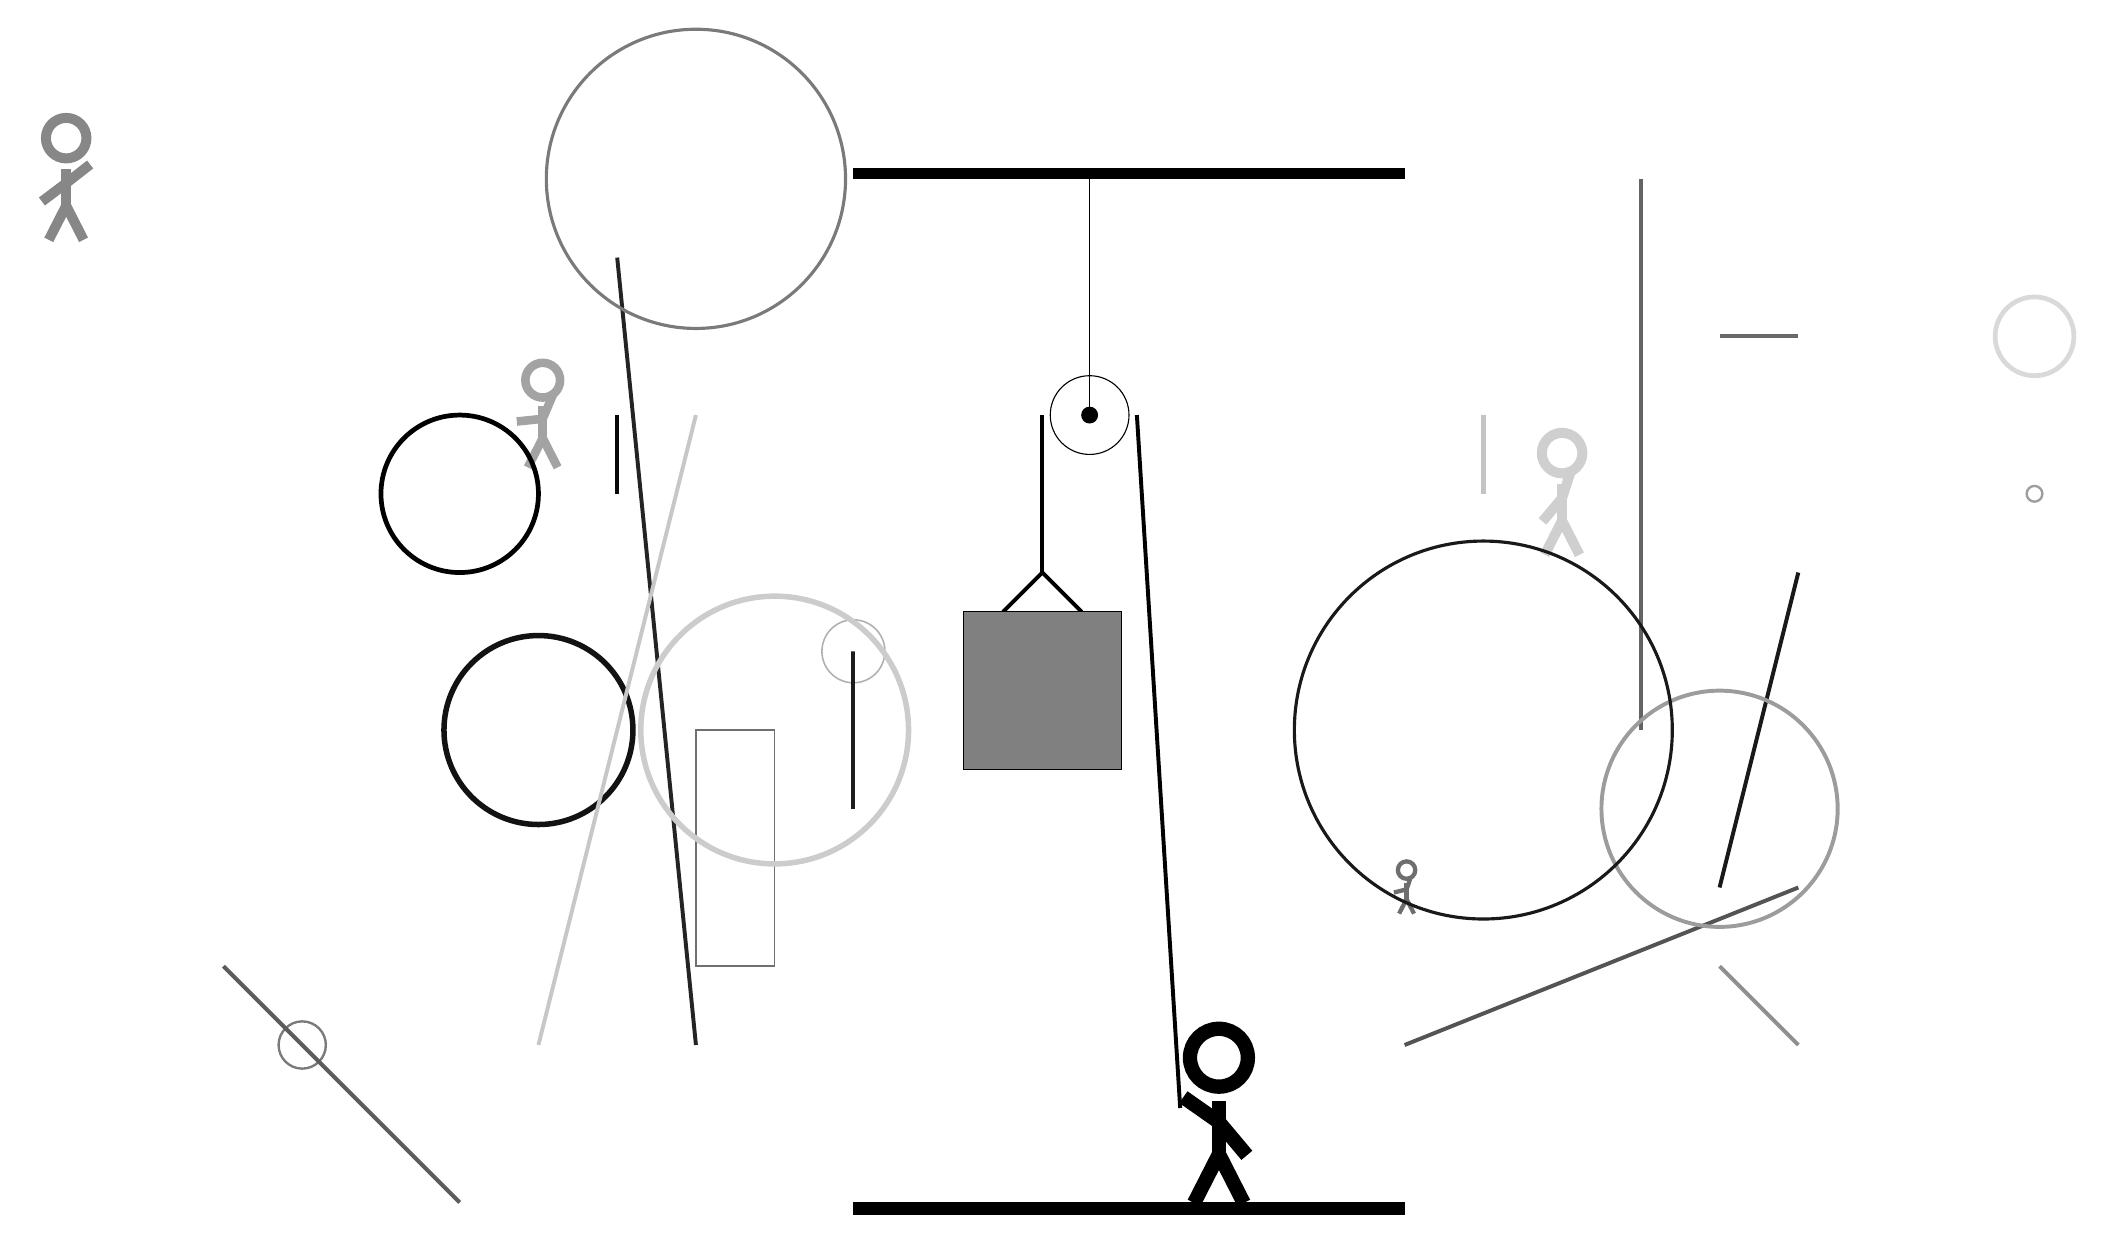
\begin{tikzpicture}
		%%%%% START %%%%%
		
		\draw[fill=black] (-2, 10) rectangle (5, 10.125);
		
		\draw (1, 7) circle (0.5);
		\draw[fill=black] (1, 7) circle (0.1);
		\draw (1, 10) -- (1, 7);
		
		\draw[line width=0.5mm] (-0.1, 4.5) -- (0.4, 5.0) -- (0.9, 4.5);
		\draw[fill=black!50] (-0.6, 4.5) rectangle (1.4, 2.5);
		
		\draw[line width=0.5mm, color=black!61](8, 3) -- (8, 10);
		
		\draw[line width=0.7mm, color=black!23] (6, 7) rectangle (6, 6);
		\draw[line width=0.2mm, color=black!56] (-4, 3) rectangle (-3, 0);
		\draw[line width=0.5mm, color=black!59](10, 8) -- (9, 8);
		
		\draw [line width=0.2mm, color=black!31](-2, 4) circle (0.4);
		
		\draw[line width=0.5mm, color=black!86](-4, -1) -- (-5, 9);
		\draw [line width=0.4mm, color=black!32](-6, 3) circle (0.0);
		\draw[line width=0.5mm, color=black!90](9, 1) -- (10, 5);
		\draw[line width=0.5mm, color=black!67](10, 1) -- (5, -1);
		\draw[line width=0.5mm, color=black!89] (-2, 2) rectangle (-2, 4);
		\draw [line width=0.7mm, color=black!20](-3, 3) circle (1.7);
		
		\node[line width=0.2mm, color=black!47] at (-12, 10) {\Strichmaxerl[7][37][38]};
		\draw [line width=0.6mm, color=black!15](13, 8) circle (0.5);
		\node[line width=0.7mm, color=black!57] at (5, 1) {\Strichmaxerl[3][14][71]};
		\draw[line width=0.5mm, color=black!44](9, 0) -- (10, -1);
		\node[line width=0.7mm, color=black!19] at (7, 6) {\Strichmaxerl[7][50][72]};
		
		\node[line width=0.5mm, color=black!36] at (-6, 7) {\Strichmaxerl[6][6][67]};
		\draw [line width=0.3mm, color=black!52](-9, -1) circle (0.3);
		\draw[line width=0.5mm, color=black!64](-7, -3) -- (-10, 0);
		\draw [line width=0.7mm, color=black!93](-6, 3) circle (1.2);
		\draw [line width=0.5mm, color=black!39](9, 2) circle (1.5);
		\draw [line width=0.3mm, color=black!38](13, 6) circle (0.1);
		
		\draw [line width=0.4mm, color=black!90](6, 3) circle (2.4);
		\draw[line width=0.5mm, color=black!97](-5, 7) -- (-5, 6);
		\draw [line width=0.6mm, color=black!100](-7, 6) circle (1.0);
		
		\draw[line width=0.5mm, color=black!22](-4, 7) -- (-6, -1);
		
		\draw [line width=0.4mm, color=black!52](-4, 10) circle (1.9);
		
		\draw[line width=0.5mm] (0.4, 7) -- (0.4, 5.0);
		\centerarc[line width=0.5mm](1, 7)(0:180:0.6);
		\draw[line width=0.5mm](1.6, 7) -- (2.15, -1.8);
		
		\node at (2.6, -1.9) {\Strichmaxerl[10][-35][-50]};
		
		\draw[fill=black] (-2, -3) rectangle (5, -3.15);
		
		%%%%% END %%%%%
	\end{tikzpicture}
\end{document}